% Slides for the PyPSA Labs / Google "Catalyst" project (SOW WP2: 2025
% techno-economic baseline). Figures come from ../tech/figures/slides/, the
% 16:9 layout of the cost-baseline workflow; run the tech workflow first or
% `snakemake -c1` here, which does both. Template: PyPSA Labs beamer theme
% (copied from beamer/); the template's demonstration slides are kept at the
% back as a style reference.
\documentclass[11pt,aspectratio=169,t]{beamer}
\usetheme{PyPSALabs}

% LICENCE (also puts the icon on the title page and in the footline)
\usepackage[type={CC},modifier={by},version={4.0}]{doclicense}
\usepackage{array}   % ragged-right p-columns in the timeline table
\usepackage{multicol} % two-column references slide
% generated by make_references.py -- reference numbers by key
\newcommand{\reftd}{1}
\newcommand{\refdea}{2}
\newcommand{\refdiw}{3}
\newcommand{\reflazard}{4}
\newcommand{\refatb}{5}
\newcommand{\refpnnl}{6}
\newcommand{\refeia}{7}
\newcommand{\refliftoffnuclear}{8}
\newcommand{\refliftoffgeo}{9}
\newcommand{\refnrelegs}{10}
\newcommand{\refbnef}{11}
\newcommand{\reffervo}{12}
\newcommand{\refnetpower}{13}
\newcommand{\refenergydome}{14}
\newcommand{\refform}{15}
\newcommand{\refbloom}{16}
\newcommand{\refprojects}{17}
\newcommand{\refpriam}{18}
\newcommand{\refsow}{19}
      % \ref<key> = reference number, generated from references.yaml

% REFERENCES
\usepackage[style=nature, doi=true, maxcitenames=3, backend=biber]{biblatex}
\addbibresource{slides.bib}
\renewcommand*{\bibfont}{\footnotesize}

% GRAPHICS
\graphicspath{{figures/}{screenshots/}{./}}

% a figure that may be wider than the text block, centred on the page
\newcommand{\wideimage}[2][15.2cm]{%
  \makebox[\textwidth][c]{\includegraphics[width=#1]{#2}}}

% like the theme's \source, but wider and two lines high (up to the logo)
\newcommand{\sourcewide}[1]{\begin{textblock*}{10.9cm}(2.2cm,8.0cm)%
  {\tiny\usebeamercolor[fg]{framesource}%
   \setlength{\parskip}{0pt}\raggedright #1\par}%
\end{textblock*}}

% TIMELINE SLIDE helpers (TikZ; macros with arguments cannot be defined inside a frame)
\newcommand{\wpbar}[5]{% row, start month, end month (inclusive), colour, label (left column)
  \fill[#4, rounded corners=2pt] (#2-1,-#1+0.3) rectangle (#3,-#1-0.3);
  \node[anchor=east, text=branddark, font=\scriptsize] at (-0.3,-#1) {#5};}
\newcommand{\msmark}[3]{% month, row, short label above the tick
  \draw[branddark, line width=1.2pt] (#1,-#2+0.42) -- (#1,-#2-0.42);
  \node[anchor=south, text=branddark, font=\tiny\bfseries, inner sep=1pt] at (#1,-#2+0.42) {#3};}

% TITLE PAGE
\title{Catalytic Impact of Early Investments in Advanced Clean Energy Technologies}
\subtitle{Kick-off}

\author{}
\institute{PyPSA Labs, Google}
% both partner logos on the title page, PyPSA Labs above Google. Both PNGs have
% the same 3:1 aspect ratio, so equal widths give equal heights; the minipage
% centres them on a common axis.
\titlegraphic{\begin{minipage}{4.2cm}\centering
  
\includegraphics[width=4.2cm]{logo}\\[0.9cm]
  
\includegraphics[width=4.2cm]{google_logo}
\end{minipage}}

\date{8 September 2026}

\begin{document}

\begin{frame}[plain]
  \titlepage
\end{frame}
\addtocounter{framenumber}{-1}


% PROJECT OVERVIEW: project objective above a compact archetype map
\begin{frame}{Project overview}
  \footnotesize
  \vspace{-0.2cm}
  \begin{itemize}\setlength{\itemsep}{0.3em}
    \item Lay the foundation for understanding the \alert{catalytic impact of early investments} in advanced clean electricity technologies
    \item Quantitative illustration of the \alert{direct and indirect} system-wide emissions reductions and cost-decline trajectories
    \item Inform \alert{consequential and out-of-scope emissions accounting methodologies} and the broader conversation on how early-mover investments should be valued
    \item Deliver an \alert{open-source, reproducible scientific workflow}
  \end{itemize}
  % Compact crop preserves geographic context without competing with the objective.
  \begin{textblock*}{\paperwidth}(0cm,5.95cm)
    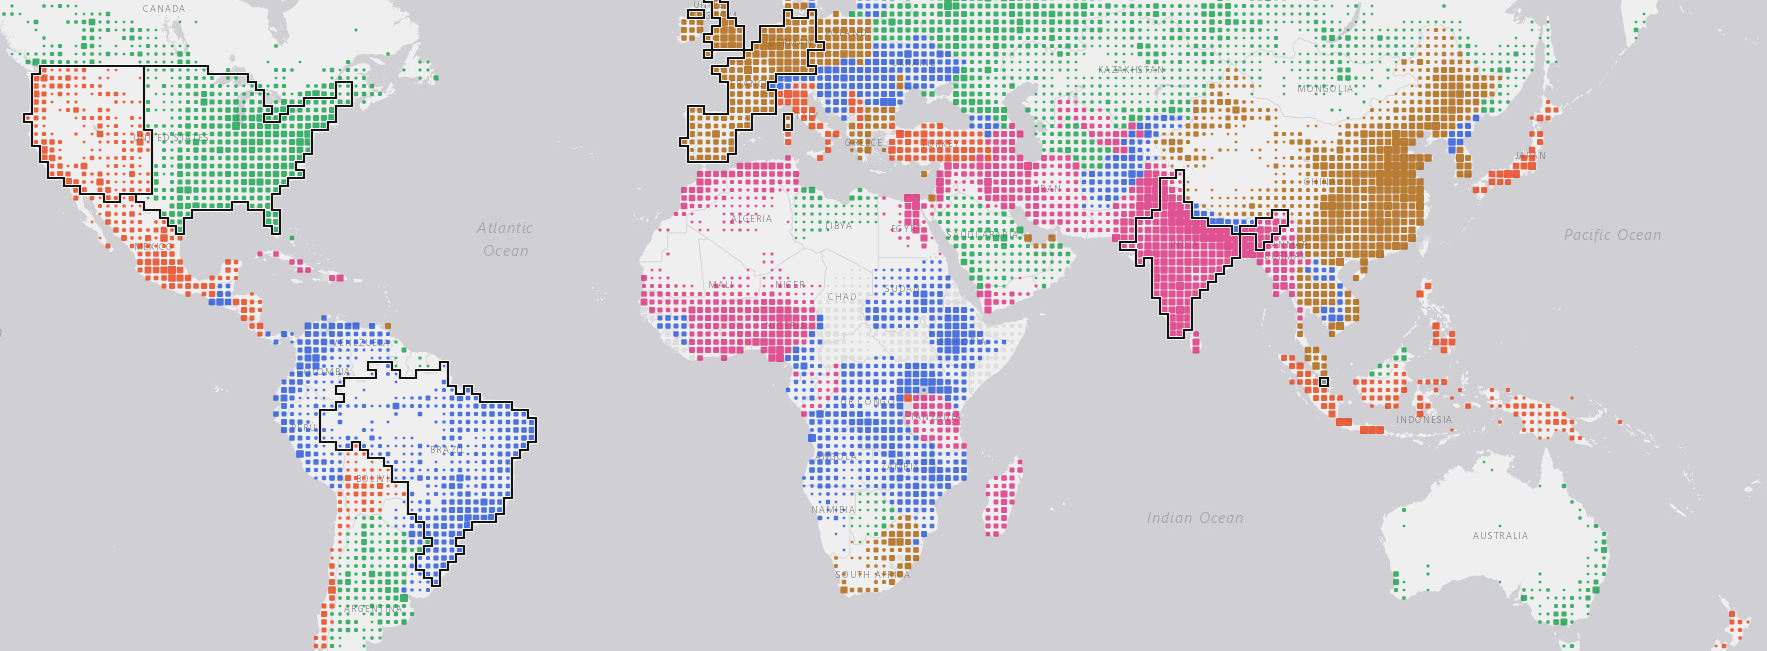
\includegraphics[width=\paperwidth, height=2.0cm, trim=0 120px 0 110px, clip]{map_screenshot}
  \end{textblock*}
\end{frame}

% MODELLING APPROACH: bullets on the left, PyPSA-Eur network plot on the right
\begin{frame}{Modelling setup 1/2}
  \begin{columns}[T]
    \begin{column}{0.55\textwidth}
      \small
      \begin{itemize}\setlength{\itemsep}{0.3em}
        \item \alert{PyPSA} for capacity expansion and dispatch optimisation
        \item \alert{PyPSA-Earth} as the global data pipeline: brownfield fleet, demand, grid topology
        \item \alert{atlite} for renewable resource potentials and capacity factors
        \item Representative regions \alert{\textit{aka grid} archetypes} featuring jurisdictions with varying grid topologies, renewable resource potentials, technology portfolios, etc.
      \end{itemize}
    \end{column}
    \begin{column}{0.45\textwidth}
      \centering
      \vspace{0.3cm}
      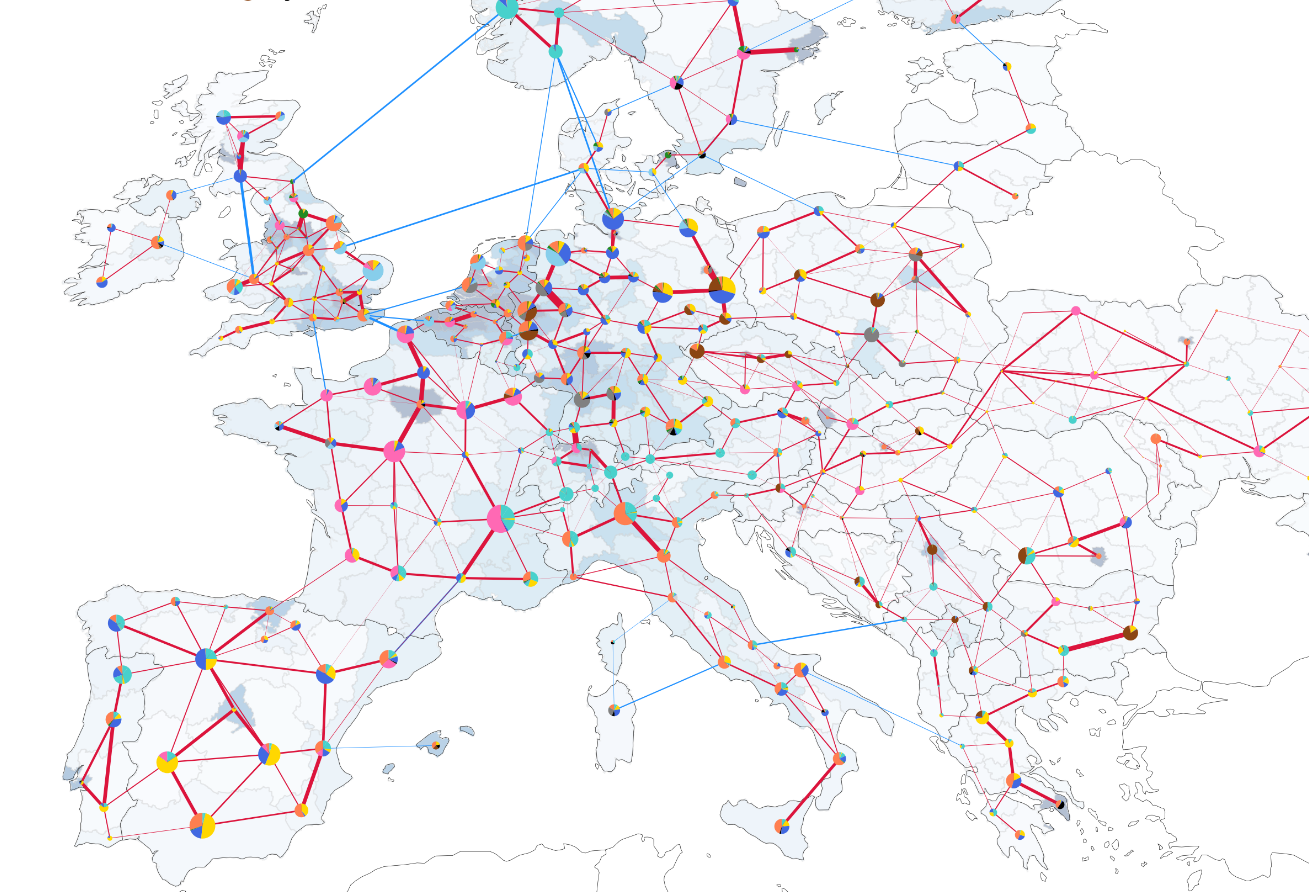
\includegraphics[width=\linewidth]{pypsa-eur}
    \end{column}
  \end{columns}
\end{frame}

% CATALYTIC INVESTMENT: bullets on the left, feedback-loop figure from the Joule paper on the right
\begin{frame}{Modelling setup 2/2}
  \begin{columns}[T]
    \begin{column}{0.55\textwidth}
      \footnotesize
      \vspace{-0.2cm}
      \begin{itemize}\setlength{\itemsep}{0.35em}
        \item Use 2025 as a \alert{validation year}
        \item Run a \alert{capacity-expansion model} for each grid archetype across investment years from 2025 to 2050
        \item Clear markets for advanced technologies between investment years; learning curves pass updated costs forward \alert{myopically}
        \item Compare a \alert{benchmark scenario} without catalytic action with a scenario including action by early investors
        \item Like-for-like comparison in system metrics (e.g. avoided emissions) to quantify impact of catalytic action
      \end{itemize}
    \end{column}
    \begin{column}{0.5\textwidth}
      \centering
      \vspace{0.3cm}
      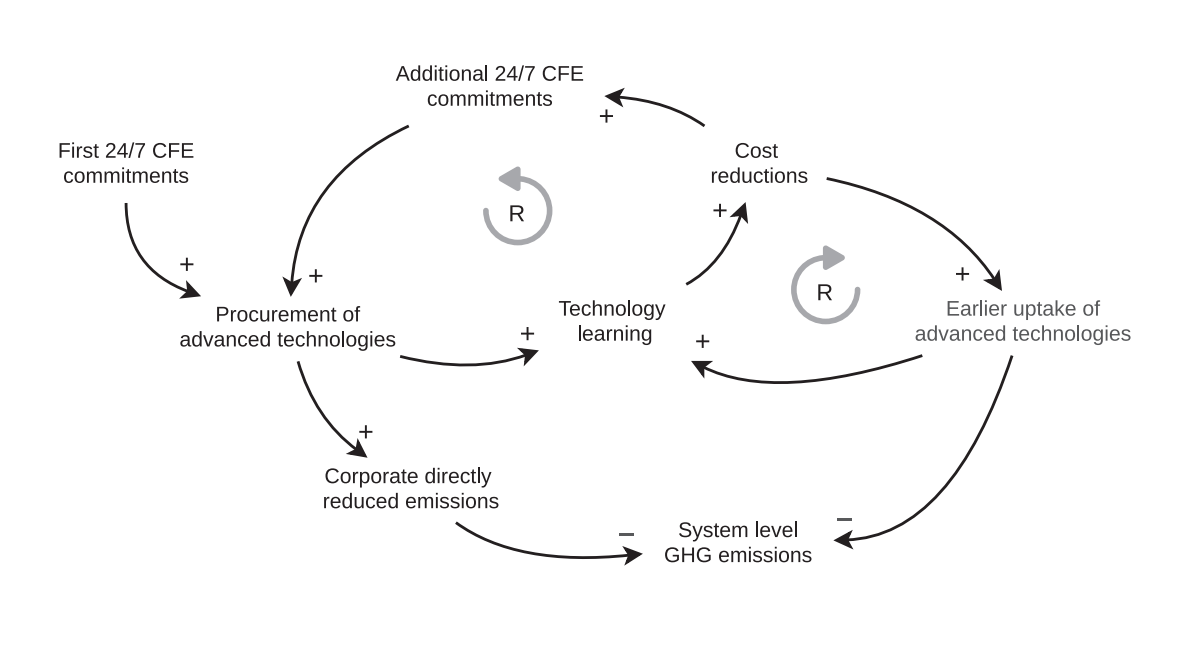
\includegraphics[width=\linewidth]{riepin_catalytic_investment}
    \end{column}
  \end{columns}
\end{frame}

\begin{frame}{Scenarios}
  \vspace{-0.35cm}
  \begin{columns}[T]
    \begin{column}{0.48\textwidth}
      \footnotesize
      \textbf{\alert{S1 --- Reference pathway}}\par
      Each archetype follows current cost trajectories and announced retirements, without catalytic investment. \alert{Establishes the counterfactual baseline} for all impact estimates.
    \end{column}
    \begin{column}{0.48\textwidth}
      \footnotesize
      \textbf{\alert{S2 --- Catalytic early investment}}\par
      Corporate and institutional buyers directly procure advanced clean technologies, with investment scale anchored to a share of regional demand and the portfolio optimised for local system needs. \alert{Early deployment accelerates learning and cost competitiveness} beyond buyers' regions.
    \end{column}
  \end{columns}

  \vspace{0.1cm}
  {\scriptsize\textbf{Additional scenarios} represent alternative futures to baseline.}
  \vspace{-0.15cm}
  \begin{columns}[T]
    \begin{column}{0.49\textwidth}
      \tiny
      \begin{itemize}\setlength{\itemsep}{0.2em}
        \item \gr{Wind/solar acceptance limits:} tighter land-use, protected-area and social-acceptance constraints increase the value of clean firm power.
        \item \gr{CDR breakthrough:} engineered removal reaches about 150 EUR/tCO\textsubscript{2} by 2040, making gas plus CDR a competitive backup option.
        \item \gr{Advanced baseload breakthrough:} rapid FOAK-to-commercial cost decline for SMRs or another firm clean technology.
      \end{itemize}
    \end{column}
    \begin{column}{0.49\textwidth}
      \tiny
      \begin{itemize}\setlength{\itemsep}{0.2em}
        \item \gr{Advanced geothermal breakthrough:} commercial success in geologically suitable regions creates locally significant catalytic impact.
        \item \gr{SOFC breakthrough:} enable cheap, efficient backup running on hydrogen or natural gas with high CO\textsubscript{2} capture; reduces the premium for LDES and flexible clean generation.
      \end{itemize}
    \end{column}
  \end{columns}
\end{frame}


% Gantt of the four SOW work packages (left) and the milestone list (right).
% Month 1 is taken as September 2026 (SOW effective date = last signature).
\newcommand{\tlstart}{Sep 2026}
\begin{frame}{SOW work packages and milestones}
  \begin{columns}[T]
    \begin{column}{0.52\textwidth}
      \vspace{0.3cm}
      \begin{tikzpicture}[x=0.33cm, y=0.72cm, font=\scriptsize]
        % month grid with calendar months
        \foreach \m in {1,...,12} {
          \draw[branddark!15] (\m-1,0.55) -- (\m-1,-4.6);
          \node[anchor=south, text=branddark!65, font=\tiny] at (\m-0.5,0.55) {\m};
        }
        \foreach \m/\l in {1/Sep,4/Dec,7/Mar,10/Jun} {
          \node[anchor=north west, text=branddark!50, font=\tiny, inner xsep=1pt] at (\m-1,0.55) {\l};
        }
        \draw[branddark!15] (12,0.55) -- (12,-4.6);
        \node[anchor=east, text=branddark!65, font=\tiny] at (-0.3,0.85) {month};
        % work packages
        \wpbar{1}{1}{3}{brandblue}{WP1 Data \& RE workflow}
        \wpbar{2}{4}{6}{pypsagreen}{WP2 Techno-economics}
        \wpbar{3}{4}{9}{brandblue!70}{WP3 Model \& scenarios}
        \wpbar{4}{10}{12}{pypsared!85}{WP4 Synthesis}
        % milestones as ticks at the end of the month
        \msmark{3}{1}{M3}
        \msmark{4}{2}{M4}
        \msmark{6}{2}{M6}
        \msmark{9}{3}{M9}
        \msmark{12}{4}{M12}
        % today
        \draw[pypsared, dashed] (0.25,0.55) -- (0.25,-4.6)
          node[below, font=\tiny, text=pypsared] {today};
        \node[anchor=north west, font=\tiny, text=branddark!55] at (1.2,-4.75)
          {M1 = \tlstart{} assumed; SOW [\refsow]: 12 months from signature};
      \end{tikzpicture}
    \end{column}
    \begin{column}{0.48\textwidth}
      \vspace{0.35cm}
      {\scriptsize\setlength{\parskip}{0pt}\renewcommand{\arraystretch}{1.25}%
      \begin{tabular}{@{}l@{\hspace{0.5em}}>{\raggedright\arraybackslash}p{5.3cm}@{}}
        \textbf{M3} \gray{Nov} & archetypes \& region mapping fixed; atlite/ERA5 feed-in with exclusion layers \\
        \textbf{M4} \gray{Dec} & calibrated data pipeline; advanced-tech parametrisation \& learning model \\
        \textbf{M6} \gray{Feb} & archetype model end-to-end, learning loop across investment years \\
        \textbf{M9} \gray{May} & full scenario suite solved 2025--2040; post-processing \& visualisation \\
        \textbf{M12} \gray{Aug} & study published; code released under open licence \\
      \end{tabular}}
    \end{column}
  \end{columns}
\end{frame}

\begin{statement}
  Prototype: Endogenous learning in the world model
\end{statement}

\begin{frame}{Prototype: Endogenous learning in the world model}
  \centering
  \wideimage{figures/learning_curve}
  \source{\url{https://github.com/nworbmot/priam-myopic}}
\end{frame}

\begin{statement}
  Open questions
\end{statement}

\begin{frame}[c]{Open questions}
  \begin{itemize}
    \item Technology palette
    \item Initial investment mechanism
    \item Modelled regions
  \end{itemize}
\end{frame}

% TECHNOLOGY PALETTE (SOW §1.2): mature = exogenous DEA/technology-data costs,
% advanced = endogenous learning in the investment loop; keep in step with
% ../tech/config.yaml
\begin{frame}{Technology palette}
  \begin{columns}[T]
    \begin{column}{0.47\textwidth}
      \begin{block}{Mature: exogenous costs}
        \footnotesize
        \begin{itemize}\setlength{\itemsep}{0.15em}
          \item Solar PV, onshore/offshore wind
          \item Hydro: reservoir, run-of-river, pumped hydro
          \item Biomass
          \item Nuclear (large LWR)
          \item Gas CCGT and OCGT
          \item Li-ion battery
        \end{itemize}
      \end{block}
    \end{column}
    \begin{column}{0.47\textwidth}
      \begin{exampleblock}{Advanced: endogenous learning}
        \footnotesize
        \begin{itemize}\setlength{\itemsep}{0.15em}
          \item LDES: CO\textsubscript{2} battery, iron-air battery, H\textsubscript{2} + SOFC, vanadium flow
          \item Nuclear SMR
          \item Next-gen geothermal
          \item Allam-cycle gas + CCS / CCGT with post-combustion capture
          \item CDR: direct air capture, cost cut-off
        \end{itemize}
      \end{exampleblock}
    \end{column}
  \end{columns}
\end{frame}

\begin{frame}{The Initial Investment Mechanism}
  \centering
  \wideimage[9cm]{screenshots/investment_mechanism}
  \vspace{-0.35cm}
  \begin{itemize}\footnotesize\setlength{\itemsep}{0.15em}
    \item Generalise the initial action beyond 24/7 CFE to represent \alert{multiple forms of catalytic investment}
    \item Let the model select the \alert{locally appropriate technology portfolio}, rather than prescribing which technologies are procured
    \item Test two mechanisms with endogenous portfolio selection: a \alert{demand-linked procurement target} and a \alert{green-premium budget}
  \end{itemize}
\end{frame}

% ARCHETYPE SLIDES: screenshots placed with textblocks (page is 16 x 9 cm; body
% from ~1.8 cm below the title to ~8.1 cm above the footline)
% SOW §1.2 illustrative archetypes on the left, the set we ended up with on the right
\begin{frame}{Modelled regions and grid archetypes}
  \begin{columns}[T]
    \begin{column}{0.56\textwidth}
      \small\textbf{Archetypes proposed in the SOW}\\[0.6em]
      \scriptsize
      \begin{itemize}\setlength{\itemsep}{0.5em}
        \item \textbf{Renewables-constrained, high-density:} Western Europe, South Korea, Japan
        \item \textbf{Geothermal-favourable:} US West, South-East Asia, Turkey, Italy
        \item \textbf{Islanded / weakly interconnected:} Western Australia, Ireland
        \item \textbf{Hydro-rich:} Norway, Brazil, parts of Canada
        \item \textbf{Fossil-heavy brownfield with large economies:} parts of the US and Europe, India
      \end{itemize}
    \end{column}
    \begin{column}{0.40\textwidth}
      \small\textbf{Archetypes and regions selected}\\[0.7em]
      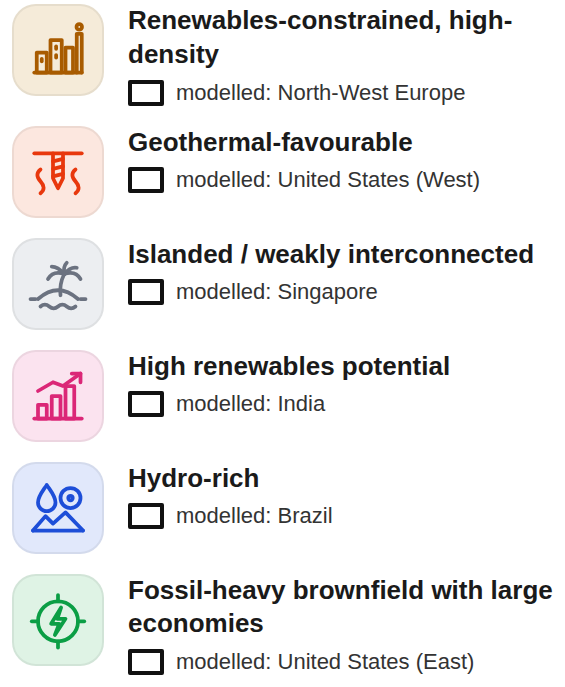
\includegraphics[height=4.8cm]{archetypes}
    \end{column}
  \end{columns}
\end{frame}

% how the archetypes were derived: the seven k-means features (scripts/sep/cluster_tsne.py) and
% the t-SNE view of the KMeans tab of the front-end (screenshots/tsne.png)
\begin{frame}{$k$-means for archetype classification}
  \begin{columns}[T]
    \begin{column}{0.47\textwidth}
      \scriptsize
      \begin{itemize}\setlength{\itemsep}{0.4em}
        \item \textbf{Autarky:} 1 at zero trade, 0 at $|$net imports$|$ $\geq 20\,\%$ of demand
        \item \textbf{Population density:} $\log_{10}$ people per km$^2$
        \item \textbf{2050 demand per capita:} $\log_{10}$ kWh per person
        \item \textbf{Demand growth to 2050:} $\log_2$ of 2050 over today's demand
        \item \textbf{Clean incumbent share:} hydro + nuclear, \% of generation
        \item \textbf{Fossil share:} coal, gas and oil, \% of generation
        \item \textbf{Geothermal potential:} installed capacity, EGS-suitable land, temperature at 5\,km
      \end{itemize}
    \end{column}
    \begin{column}{0.51\textwidth}
      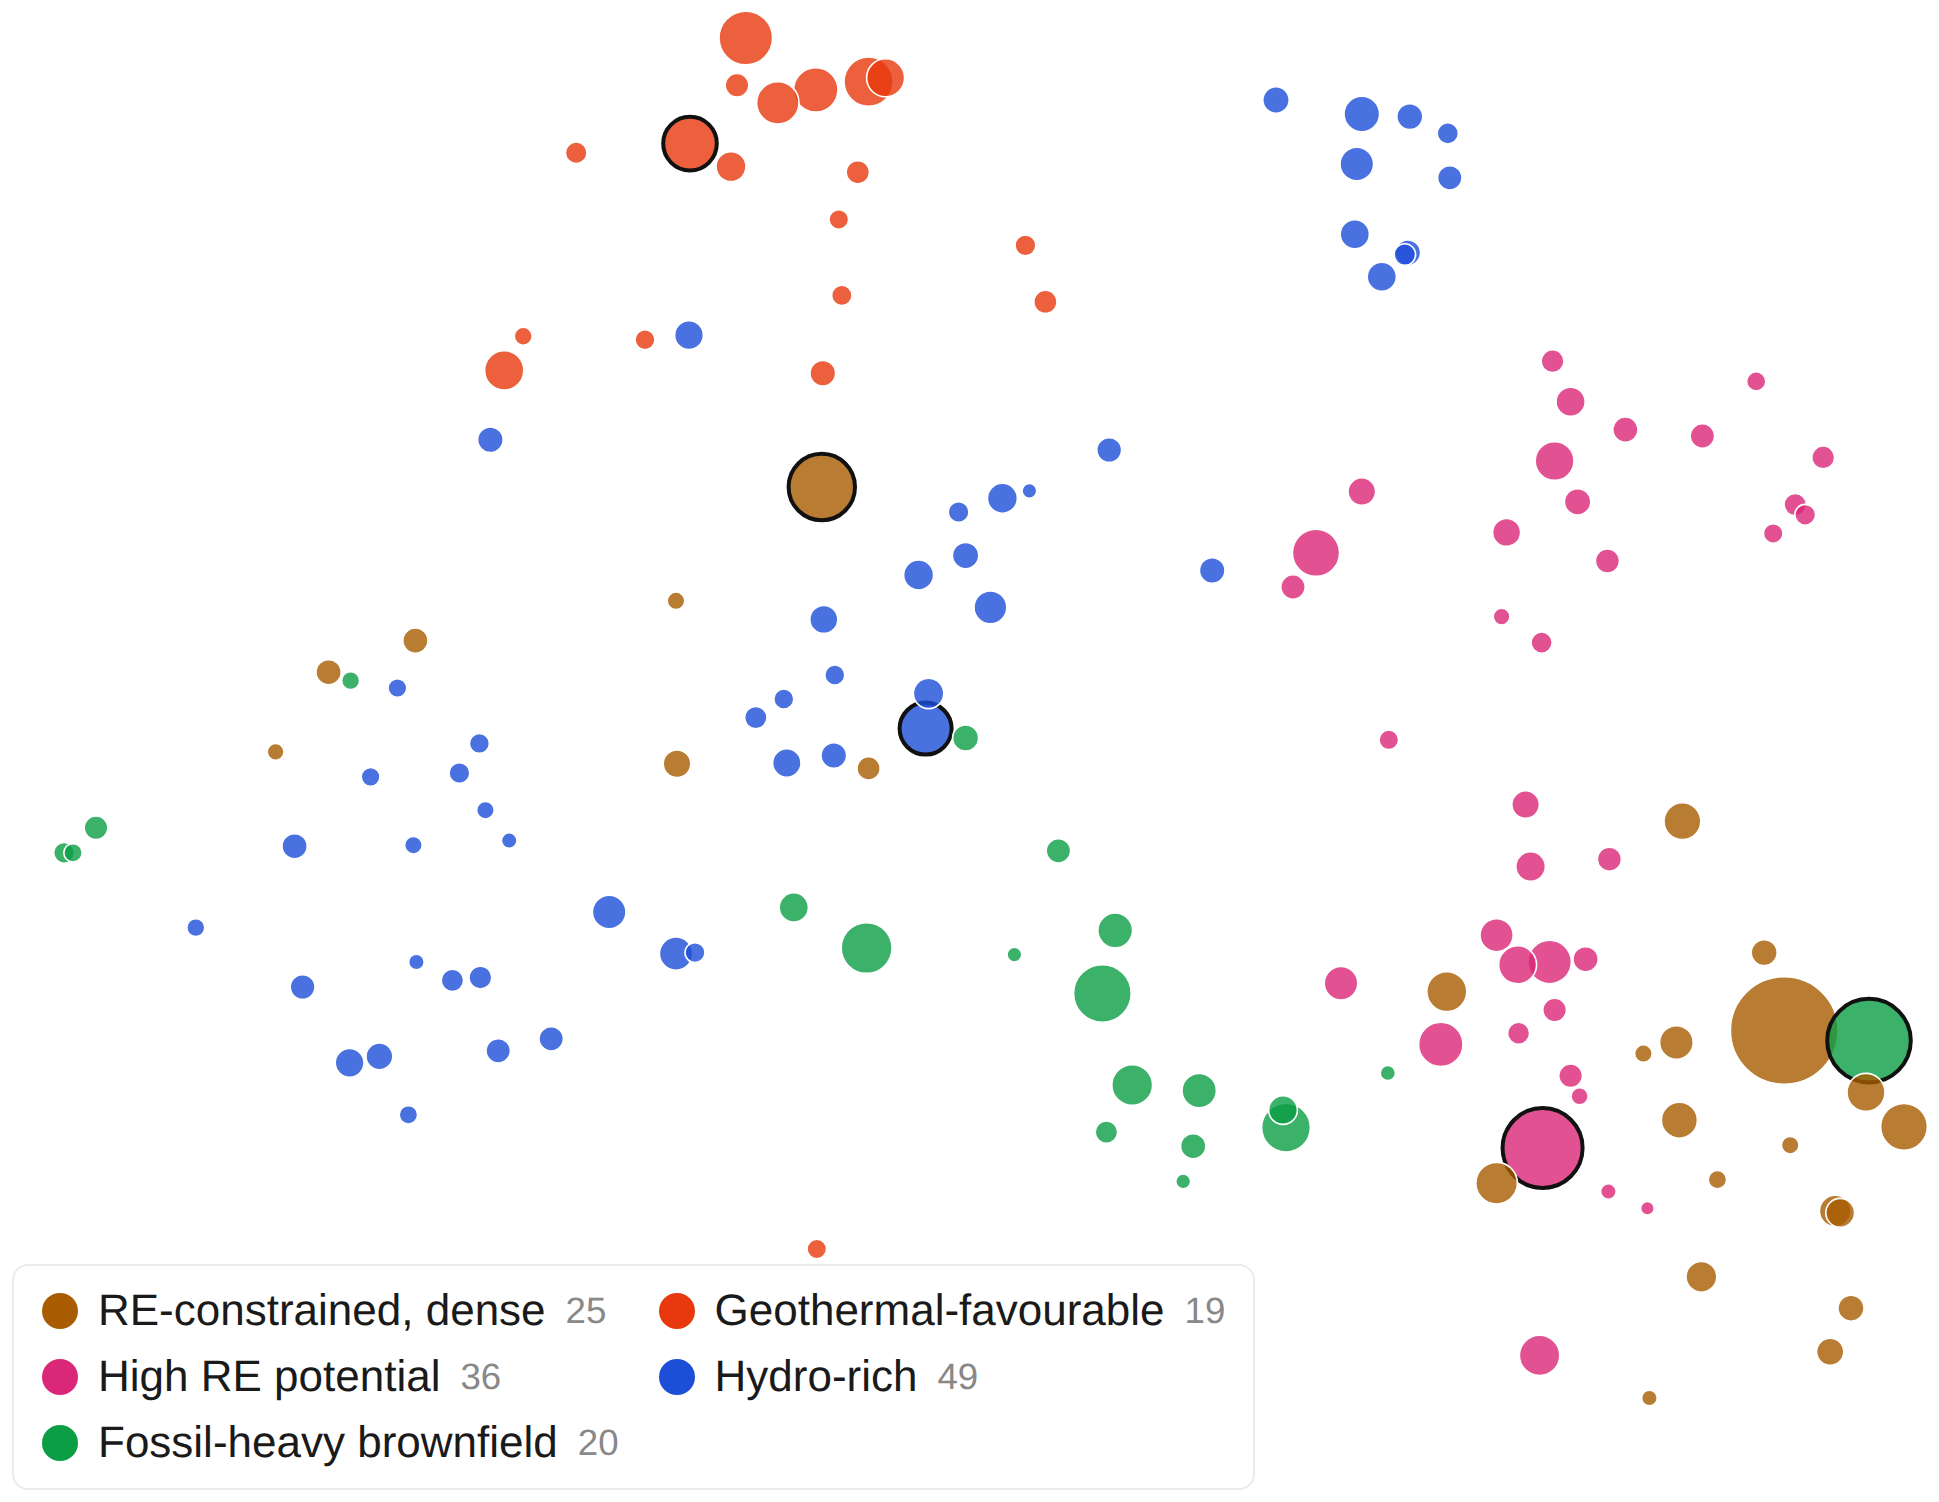
\includegraphics[width=\linewidth]{tsne}
    \end{column}
  \end{columns}
\end{frame}

\begin{frame}{Modelled regions and grid archetypes}
  \begin{textblock*}{6cm}(1cm,2.3cm)
    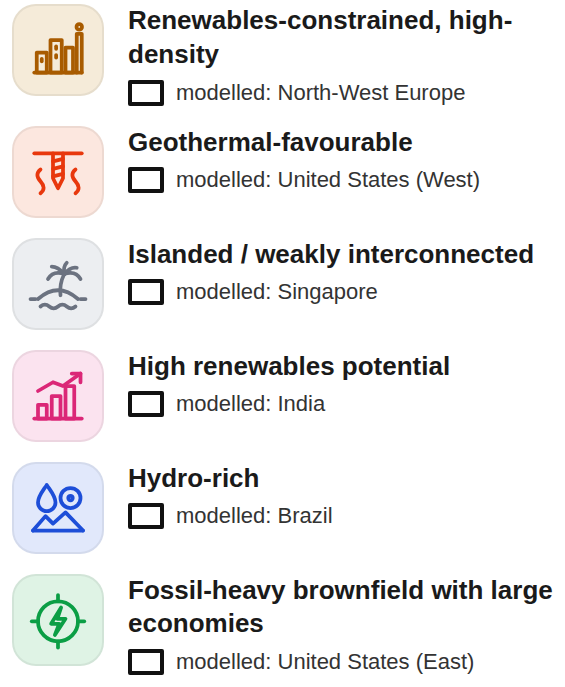
\includegraphics[height=4.8cm]{archetypes}
  \end{textblock*}
  % the map is 2.7:1, so it runs from the archetype list to the right page edge
  \begin{textblock*}{9.2cm}(6.2cm,3.0cm)
    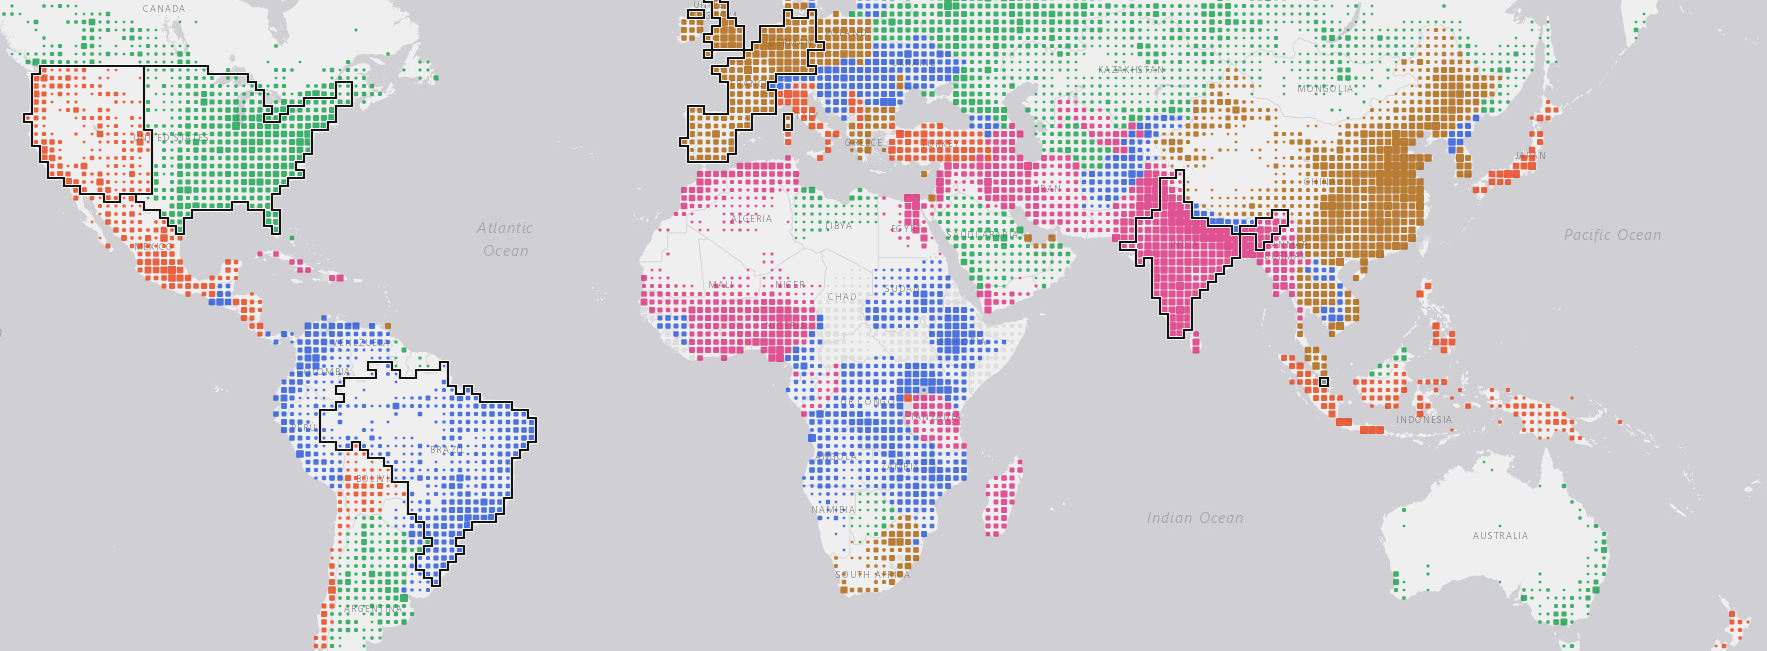
\includegraphics[width=9.2cm]{map_screenshot}
  \end{textblock*}
\end{frame}

\begin{frame}{Modelled regions and grid archetypes}
  \begin{textblock*}{6cm}(1cm,2.3cm)
    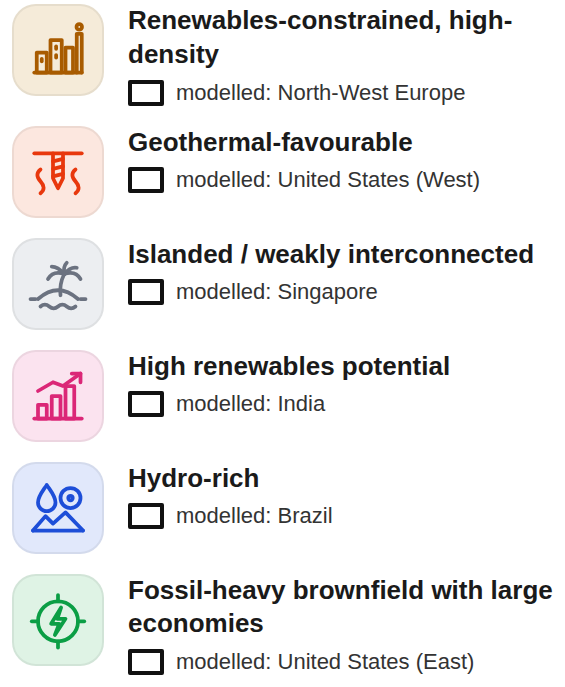
\includegraphics[height=4.8cm]{archetypes}
  \end{textblock*}
  \begin{textblock*}{6cm}(8.6cm,2.3cm)
    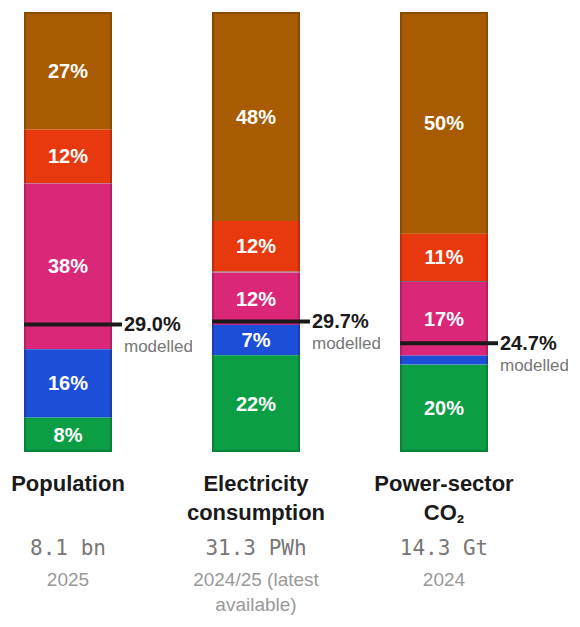
\includegraphics[height=4.8cm]{shares}
  \end{textblock*}
\end{frame}


\begin{statement}
  Annex
\end{statement}


\begin{frame}{2025 capex baseline: mature generation}
  \centering
  \wideimage{figures/capex_generation_mature}
\end{frame}

\begin{frame}{2025 capex baseline: advanced generation}
  \centering
  \wideimage{figures/capex_generation_advanced}
\end{frame}

\begin{frame}{2025 capex baseline: mature storage}
  \centering
  \wideimage{figures/capex_storage_mature}
\end{frame}

\begin{frame}{2025 capex baseline: advanced storage}
  \centering
  \wideimage{figures/capex_storage_advanced}
\end{frame}




\begin{frame}[t]{References}
  \vspace{-0.2cm}
  % generated by make_references.py from references.yaml -- do not edit
\begin{multicols}{2}\tiny\setlength{\parskip}{0.6pt}\raggedright
\noindent\hangindent=2.2em\hangafter=1\makebox[2.2em][l]{\textbf{[1]}}PyPSA, technology-data v0.15.0 (2025), cost assumptions for 2025 \gray{\href{https://github.com/PyPSA/technology-data}{github.com}}\par
\noindent\hangindent=2.2em\hangafter=1\makebox[2.2em][l]{\textbf{[2]}}Danish Energy Agency, Technology Data catalogues: electricity generation; energy storage (2024/25) \gray{\href{https://ens.dk/en/analyses-and-statistics/technology-data}{ens.dk}}\par
\noindent\hangindent=2.2em\hangafter=1\makebox[2.2em][l]{\textbf{[3]}}Schröder et al. (DIW Berlin), Costs of Electricity Generation until 2050, Data Documentation 68 (2013) \gray{\href{https://www.diw.de/documents/publikationen/73/diw_01.c.424566.de/diw_datadoc_2013-068.pdf}{diw.de}}\par
\noindent\hangindent=2.2em\hangafter=1\makebox[2.2em][l]{\textbf{[4]}}Lazard, Levelized Cost of Energy+ (LCOE+), June 2025 and v16.0 (2023) \gray{\href{https://www.lazard.com/research-insights/levelized-cost-of-energyplus/}{lazard.com}}\par
\noindent\hangindent=2.2em\hangafter=1\makebox[2.2em][l]{\textbf{[5]}}NREL, Annual Technology Baseline 2024, electricity (v3 data) \gray{\href{https://atb.nrel.gov/electricity/2024}{atb.nrel.gov}}\par
\noindent\hangindent=2.2em\hangafter=1\makebox[2.2em][l]{\textbf{[6]}}PNNL / DOE, 2022 Grid Energy Storage Technology Cost and Performance Assessment (Viswanathan et al.) \gray{\href{https://www.pnnl.gov/projects/esgc-cost-performance}{pnnl.gov}}\par
\noindent\hangindent=2.2em\hangafter=1\makebox[2.2em][l]{\textbf{[7]}}EIA / Sargent \& Lundy, Capital Cost and Performance Characteristics for Utility-Scale Generating Technologies (AEO2025) \gray{\href{https://www.eia.gov/analysis/studies/powerplants/capitalcost/}{eia.gov}}\par
\noindent\hangindent=2.2em\hangafter=1\makebox[2.2em][l]{\textbf{[8]}}US DOE, Pathways to Commercial Liftoff: Advanced Nuclear (Sep 2024 update) \gray{\href{https://liftoff.energy.gov/advanced-nuclear/}{liftoff.energy.gov}}\par
\noindent\hangindent=2.2em\hangafter=1\makebox[2.2em][l]{\textbf{[9]}}US DOE, Pathways to Commercial Liftoff: Next-Generation Geothermal Power (Mar 2024) \gray{\href{https://liftoff.energy.gov/next-generation-geothermal-power/}{liftoff.energy.gov}}\par
\noindent\hangindent=2.2em\hangafter=1\makebox[2.2em][l]{\textbf{[10]}}NREL, Enhanced Geothermal Shot Analysis for the Geothermal Technologies Office (2023) \gray{\href{https://www.nrel.gov/docs/fy23osti/84822.pdf}{nrel.gov}}\par
\noindent\hangindent=2.2em\hangafter=1\makebox[2.2em][l]{\textbf{[11]}}BloombergNEF, Energy Storage System Cost Survey 2024 (as reported by Energy-Storage.news) \gray{\href{https://about.bnef.com/}{about.bnef.com}}\par
\noindent\hangindent=2.2em\hangafter=1\makebox[2.2em][l]{\textbf{[12]}}Fervo Energy, Form S-1 registration statement (2026), Cape Station cost disclosures \gray{\href{https://www.sec.gov/}{sec.gov}}\par
\noindent\hangindent=2.2em\hangafter=1\makebox[2.2em][l]{\textbf{[13]}}NET Power, Q4 2024 results and business update (10 Mar 2025), Project Permian cost estimate \gray{\href{https://ir.netpower.com/}{ir.netpower.com}}\par
\noindent\hangindent=2.2em\hangafter=1\makebox[2.2em][l]{\textbf{[14]}}Energy Dome, CO2 Battery cost and performance statements (2022--2024) \gray{\href{https://energydome.com/co2-battery/}{energydome.com}}\par
\noindent\hangindent=2.2em\hangafter=1\makebox[2.2em][l]{\textbf{[15]}}Form Energy, iron-air modelling recommendations (2023) and cost target statements \gray{\href{https://formenergy.com/}{formenergy.com}}\par
\noindent\hangindent=2.2em\hangafter=1\makebox[2.2em][l]{\textbf{[16]}}Bloom Energy, product cost disclosures 2017--2023 (via Thunder Said Energy); Energy Server datasheet (2026) \gray{\href{https://www.bloomenergy.com/}{bloomenergy.com}}\par
\noindent\hangindent=2.2em\hangafter=1\makebox[2.2em][l]{\textbf{[17]}}Developer, regulator and press disclosures of individual projects (Vogtle, Hinkley Point C, Flamanville 3, Darlington, Kemmerer, Snowy 2.0, Fengning, Dalian, Alliant, ...); per-project sources in the repository \gray{\href{https://github.com/PyPSA/pypsa-labs-google}{github.com}}\par
\noindent\hangindent=2.2em\hangafter=1\makebox[2.2em][l]{\textbf{[18]}}T. Brown, priam-myopic: myopic world electricity model with endogenous learning (prototype, 2026) \gray{\href{https://github.com/nworbmot/priam-myopic}{github.com}}\par
\noindent\hangindent=2.2em\hangafter=1\makebox[2.2em][l]{\textbf{[19]}}PyPSA Labs and Google, Statement of Work: Catalytic Impact of Early Investments in Advanced Clean Energy Technologies (2026)\par
\end{multicols}

\end{frame}


\begin{frame}{Get in touch}

  \begin{columns}[c]
    \begin{column}{0.65\textwidth}
      \textbf{Dr. Lukas Franken, Dr. Iegor Riepin, Prof. Dr. Tom Brown} \\
      \href{https://pypsalabs.org}{pypsalabs.org}
    \end{column}
    \begin{column}{0.3\textwidth}
      \raggedleft\qrcode[height=2.6cm]{https://pypsalabs.org}
    \end{column}
  \end{columns}

  % Imprint: mandatory on business letters of a GmbH/UG in electronic form
  % (§ 35a GmbHG) and on publicly available slides (§ 5 DDG, ex § 5 TMG).
  % Adjust the legal form, register entry and management to your entity.
  \legalnote{%
    PyPSA Labs gGmbH, Mertensstr. 16A, 13587 Berlin, Germany ~·~
    District Court Charlottenburg \mbox{HRB 288490 B} ~·~
    Managing Directors: Prof.~Dr.~Thomas William Brown \& Dr.-Ing.~Fabian Neumann ~·~
    \mbox{VAT ID}: pending ~·~
    \textcopyright{} 2026 The Authors ~·~ Slides and figures by the authors
    unless stated otherwise, licensed under CC BY 4.0.}
\end{frame}

\end{document}
